

\chapter{Results}

In this chapter, we describe the results from our pose and depth experiments. In the previous chapter, we suggested two pipelines for learning these tasks, as well as several input strategies that allow neural networks to ingest 4D light field data. We organise this chapter into three sections. The first two sections describe the results from each pipeline, and in the third, we compare their relative performance in order to build a quantitative basis for our discussion in the following chapter.


\section{Single-Image-Reconstruction Pipeline}


\subsection{Depth Estimates}

\subsection{Trajectories}

\section{Light-Field-Reconstruction Pipeline}


\subsection{Depth Estimates}

\begin{figure}[H]
    % \centering 
    \subfloat{
        \label{input_img_20}
        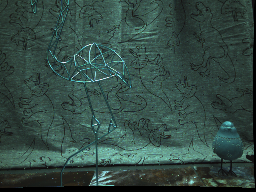
\includegraphics[width=0.19\textwidth]{images/depth/20/image.png}
    }
    \subfloat{
        \label{multiwarp_epi_20}
        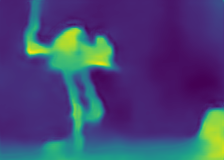
\includegraphics[width=0.19\textwidth]{images/depth/20/multiwarp_epi_20.png}
    }
    \subfloat{
        \label{multiwarp_epi_20}
        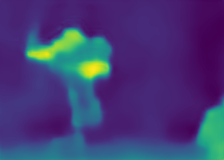
\includegraphics[width=0.19\textwidth]{images/depth/20/multiwarp_stack_20.png}
    }
    \subfloat{
        \label{multiwarp_epi_20}
        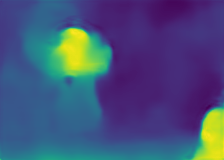
\includegraphics[width=0.19\textwidth]{images/depth/20/multiwarp_fs9_20.png}
    }
    \subfloat{
        \label{multiwarp_epi_20}
        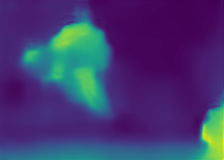
\includegraphics[width=0.19\textwidth]{images/depth/20/multiwarp_fs5_20.png}
    } \\

    \setcounter{subfigure}{0}
    \subfloat[Input Image]{
        \label{input_img_20}
        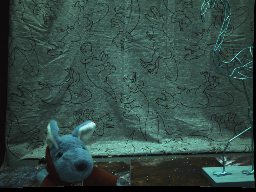
\includegraphics[width=0.19\textwidth]{images/depth/44/image.png}
    }
    \subfloat[Tiled EPIs]{
        \label{multiwarp_epi_20}
        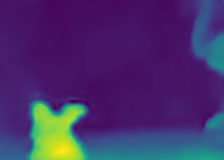
\includegraphics[width=0.19\textwidth]{images/depth/44/multiwarp_epi_44.png}
    }
    \subfloat[Volumetric Image]{
        \label{multiwarp_epi_20}
        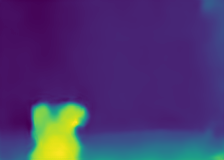
\includegraphics[width=0.19\textwidth]{images/depth/44/multiwarp_stack_44.png}
    }
    \subfloat[Focal Stack (9)]{
        \label{multiwarp_epi_20}
        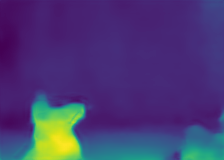
\includegraphics[width=0.19\textwidth]{images/depth/44/multiwarp_fs9_44.png}
    }
    \subfloat[Focal Stack (5)]{
        \label{multiwarp_epi_20}
        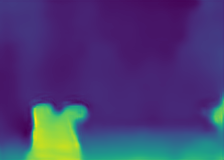
\includegraphics[width=0.19\textwidth]{images/depth/44/multiwarp_fs5_44.png}
    } \\
    
\end{figure}

\subsection{Trajectories}

\begin{figure}[H]
    \setcounter{subfigure}{0}
    % \centering 
    \subfloat[Tiled EPIs]{
        \label{input_img_20}
        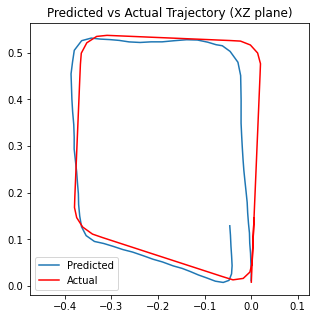
\includegraphics[width=0.5\textwidth]{images/trajectories/multiwarp-epi.png}
    } 
    \subfloat[Volumetric Image]{
        \label{multiwarp_epi_20}
        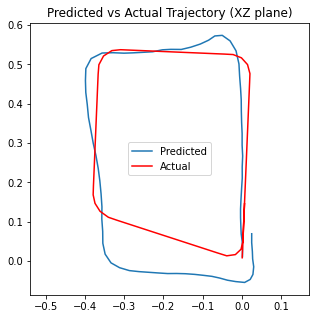
\includegraphics[width=0.5\textwidth]{images/trajectories/multiwarp-volumetric.png}
    } \\
    \subfloat[Focal Stack (9)]{
        \label{multiwarp_epi_20}
        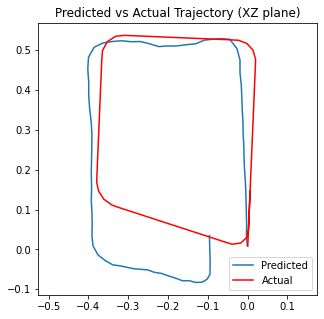
\includegraphics[width=0.5\textwidth]{images/trajectories/multiwarp-focalstack-17-9.png}
    }
    \subfloat[Focal Stack (5)]{
        \label{multiwarp_epi_20}
        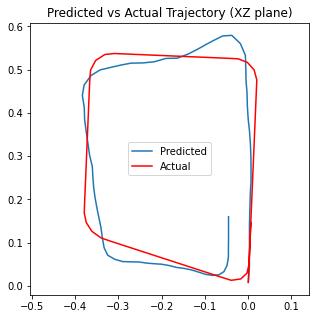
\includegraphics[width=0.5\textwidth]{images/trajectories/multiwarp-focalstack-17-5.png}
    }
    
\end{figure}

\section{Comparison between Pipelines}




